\documentclass[journal]{IEEEtran}
\IEEEoverridecommandlockouts

\usepackage{amsmath,amssymb,amsfonts}
\usepackage{graphicx}
\usepackage{booktabs}
\usepackage{url}
\usepackage{xcolor}

\newcommand{\todo}[1]{\textcolor{red}{\textbf{[TODO: #1]}}}

\DeclareMathOperator{\rank}{rank}
\newcommand{\bG}{\mathbf{G}}
\newcommand{\bS}{\mathbf{S}}
\newcommand{\bB}{\mathbf{B}}
\newcommand{\bW}{\mathbf{W}}
\newcommand{\bZ}{\mathbf{Z}}
\newcommand{\bg}{\mathbf{g}}
\newcommand{\CN}{\mathcal{CN}}
\newcommand{\Hank}{\mathcal{H}}

\begin{document}

\title{On the Evaluation of Structural Priors in Unrolled\\
Channel Estimation for Rydberg Atomic Receivers}

\author{Abdullah~Haatim%
\thanks{A.~Haatim is with the \todo{CONFIRM DEPARTMENT: taken from an earlier
draft in this project, not from a definitive source} Department of Electrical
and Electronics Engineering, Birla Institute of Technology and Science,
Pilani~--- Pilani Campus, India (e-mail:
f20220519@pilani.bits-pilani.ac.in).}}

\maketitle

\begin{abstract}
Adding an explicit structural prior to an unrolled channel estimator usually
improves the reported metric, and the improvement is usually attributed to the
prior. We show that in magnitude-only channel estimation for Rydberg atomic
receivers, most of that improvement is an artifact of how such estimators are
trained and scored. Normalized error averaged per sample over a mixed-SNR
training set puts $89.7\%$ of the gradient below $5$~dB, leaving the
high-SNR regime underfitted; a structural prior then supplies at high SNR what
training did not. Train both arms adequately and a $+1.209$~dB structural
advantage falls by a factor of fifteen, to $+0.078$~dB. The first casualty of
this control was our own structured estimator. We propose a matched-adequacy
protocol, show that simply rebalancing the loss recovers $+1.902$~dB at
SNR~$\ge5$~dB at no low-SNR cost, and show that pilot efficiency and
pilot-count generalization are distinct quantities differing by $2.231$~dB.
Results are simulation only.
\end{abstract}

\begin{IEEEkeywords}
Algorithm unrolling, channel estimation, evaluation methodology, phase
retrieval, Rydberg atomic receiver, structural priors.
\end{IEEEkeywords}

\section{Introduction}

\IEEEPARstart{U}{nrolling} an iterative estimator into a trained
network~\cite{gregor2010,monga2021} has become standard for channel estimation,
including for Rydberg atomic receivers, where the magnitude-only readout makes
the problem one of phase retrieval~\cite{xiao2026,cui2025}. A recurring next
step is to add an explicit structural prior --- a low-rank projection, a
sparsity constraint --- inside the unrolled loop, and to report the resulting
improvement as evidence that the prior supplies information the network lacks.

This paper argues that such evidence is usually not decisive, and that the
reason is a convention so widespread it is rarely stated: the training loss is
a per-sample normalized error, averaged over a training set spanning a wide
SNR range.

\textbf{This is a finding about evaluation practice, and we did not arrive at
it as critics.} We built a Hankel-structured unrolled estimator, measured a
clear $+1.209$~dB advantage at high SNR, and believed it. The control
described in Sec.~\ref{sec:protocol} was run to characterize that advantage,
not to remove it. It removed it: the same contrast under matched training
adequacy is $+0.078$~dB. The first casualty of the protocol we propose was our
own method, and we report it because a result that survives an author's
attempt to keep it is worth more than one that was never tested.

\textbf{Contributions.}
\begin{enumerate}
\item An attribution decomposition of an unrolled estimator's gain, separating
the learned filter, the attention block, and unrolling itself against a matched
non-unrolled control.
\item Identification of the confound: per-sample normalized error over mixed
SNR concentrates the gradient at low SNR, and a structural prior compensates
for the resulting high-SNR underfitting. We give a matched-adequacy protocol
that separates the two.
\item A corrected loss that is not a workaround but a fix, recovering
$+1.902$~dB at SNR~$\ge5$~dB with no low-SNR penalty.
\item A demonstration that pilot efficiency and pilot-count generalization are
distinct and are conflated by a single reported curve.
\end{enumerate}

\section{System Model and Estimator}

An $N$-element uniform linear array serves $K$ users over $P$ pilots. With
$\bG\in\mathbb{C}^{N\times K}$, pilots $\bS$, known reference beam $\bB$ and
noise $\bW$, the receiver observes magnitudes only,
\begin{equation}
\bZ=\left|\bG\bS+\bB+\bW\right|,\qquad \bW_{np}\sim\CN(0,\sigma^2).
\label{eq:fwd}
\end{equation}
Each user's channel is a sum of $L_k$ plane waves on the array manifold. The
classical baseline is an expectation--maximization Gerchberg--Saxton iteration
(EM-GS)~\cite{gerchberg1972}~\todo{VERIFY CITATION}; the unrolled estimator
(``URformer'') replaces $T$ iterations with $T$ learned layers, each a
data-consistency step followed by a learned filter, a gate, and a
Transformer block across users~\cite{xiao2026}.

We implement this estimator faithfully on the geometric ULA model of
\eqref{eq:fwd} rather than reproducing any published result: the operating
point differs, and reaching the reported behaviour required roughly four times
the stated data budget. Nothing here should be read as a reproduction or a
validation of prior work, nor as a critique of any specific paper. The
convention we examine is near-universal, and our own estimator uses it.

\textbf{The reference curve is genie-aided.} Where a reference appears, it is
an unstructured least-squares estimate formed from the \emph{true} phase of
the noiseless field. It is not a bound: it presumes information no receiver
has, and being restricted to unstructured least squares it can be passed by an
estimator that exploits channel structure --- which we in fact observe below
$5$~dB in Sec.~\ref{sec:balanced}.

\section{Attribution and the Matched-Adequacy Protocol}
\label{sec:protocol}

\subsection{Where the gain comes from}

Fig.~\ref{fig:attr} decomposes the unrolled estimator's $3.345$~dB
improvement over EM-GS. The learned per-layer filter, $980$ parameters,
contributes
% src: reports/trackD_stage2_report.md:107-110
$0.147$~dB; the attention block contributes the remaining $3.198$~dB, or
$96\%$. The filter's contribution does not grow with data --- it falls
slightly, $0.193\to0.147$~dB from $20$k to $80$k training samples --- which is
what a never-capacity-limited $980$-parameter component should do.

Unrolling is doing real work independently of attention. Against a matched
control that applies one Transformer block to a converged EM-GS estimate
rather than unrolling, the unrolled estimator gains
% src: reports/trackD_stage3_report.md:98
$0.920$~dB, CI $[+0.888,+0.988]$, winning on $86.5\%$ of trials.

\begin{figure}[!t]
\centering
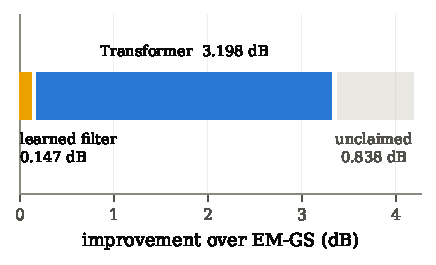
\includegraphics[width=\columnwidth]{fig/fig1_attribution.pdf}
\caption{Attribution of the unrolled estimator's gain over EM-GS at $80$k
training samples. ``Unclaimed'' is the remainder of the genie-aided
least-squares headroom, which is a reference and not a bound.}
\label{fig:attr}
\end{figure}

\subsection{The confound}

The training loss is the per-sample normalized error
$\|\hat\bG-\bG\|_F^2/\|\bG\|_F^2$, averaged over a batch drawn across the
whole SNR range. Because the normalized error of a low-SNR realization is
orders of magnitude larger than that of a high-SNR one, this average is
dominated by the low-SNR tail. Measured directly on our estimator,
% src: reports/trackD_stage5_results.json runs.C1_snr_balanced_P20.unweighted_shares
$89.7\%$ of the gradient comes from trials below $5$~dB, and the per-bin
gradient share spans a factor of $31$ across the range
(Fig.~\ref{fig:balanced}, upper panel).

The consequence is that the high-SNR regime is systematically underfitted, and
\emph{any} mechanism that improves high-SNR behaviour will appear to add
information. A structural prior is exactly such a mechanism.

\subsection{The protocol}

We propose the following control, which is cheap and which we recommend be run
before any structural prior is credited.

\begin{enumerate}
\item Measure the per-bin gradient share of the training loss. If it is far
from uniform, the regime receiving least gradient is underfitted.
\item Retrain \emph{both} the structured and unstructured arms with training
concentrated on the regime of interest, matching data budget, schedule, seed
and initialization.
\item Re-measure the contrast. What survives is attributable to the prior;
what does not was compensating for training inadequacy.
\end{enumerate}

Applying it, and reporting what it did to our own method: over $[5,20]$~dB the
structural advantage under mixed-SNR training is
% src: reports/trackD_stage4_report.md:74-78
$+1.209$~dB. Under matched focused training it is $+0.078$~dB, CI
$[+0.050,+0.112]$ --- a fifteenfold collapse (Fig.~\ref{fig:confound}). The
mechanism is visible in the absolute numbers: focused training gains the
unstructured arm $+2.653$~dB but the structured arm only $+1.629$~dB. The
unstructured network learns the array geometry by itself once it is given
adequate gradient in that regime, leaving the explicit projection little to
add.

\textbf{Scope of this negative result.} It holds at $N=32$, $K=3$, this data
budget, and the two pilot counts tested. It is not a general claim that
structural priors cannot help unrolled estimators. Indeed the same prior
applied to the \emph{classical} estimator, where no training adequacy is at
stake, gives a large and stable gain, and under a distribution shift in path
richness the structured network degrades least
% src: reports/trackD_stage5_eval.json C5_path_richness_ood
($+0.48$~dB against $+0.73$~dB). The prior buys robustness here; it is the
in-distribution accuracy claim that does not survive the control.

\begin{figure}[!t]
\centering
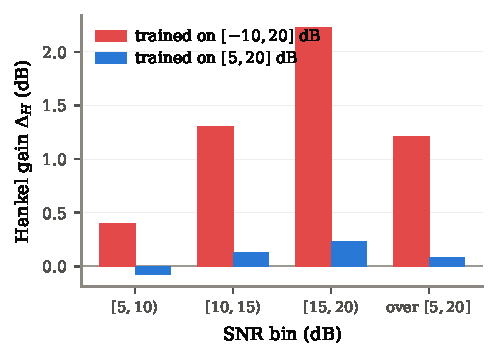
\includegraphics[width=\columnwidth]{fig/fig2_confound.pdf}
\caption{The structural gain $\Delta_H$ under mixed-SNR training and under
matched focused training. Both arms are retrained identically; only the
training SNR range differs.}
\label{fig:confound}
\end{figure}

\section{Numerical Results}
\label{sec:results}

Table~\ref{tab:params} lists the configuration. The reported statistic is the
paired per-trial median within an SNR bin, with bootstrap $95\%$ confidence
intervals over $2000$ paired test realizations.

\begin{table}[!t]
\caption{Configuration.}
\label{tab:params}
\centering
\small
\begin{tabular}{ll}
\toprule
Parameter & Value \\
\midrule
% src: trackD_urformer/config.py:120-129, 273
Array elements $N$ / users $K$ / pilots $P$ & 32 / 3 / 20 \\
Paths per user $L_k$ & $\mathcal{U}\{3,7\}$ \\
SNR (train and test) & $\mathcal{U}[-10,20]$~dB \\
Reference-to-signal ratio & 10~dB \\
Unrolled layers $T$ & 10 \\
Trainable parameters & 1{,}586{,}900 \\
% src: reports/trackD_stage2_report.md
Training samples / epochs & 80{,}000 / 13 \\
Test realizations & 2{,}000 (paired) \\
\bottomrule
\end{tabular}
\end{table}

\subsection{A corrected loss, not a workaround}
\label{sec:balanced}

The confound is a property of the loss, so we fix the loss. We weight each
sample by a static per-bin factor $w(b)=c/m(b)$, where $m(b)$ is the mean
per-sample normalized error in bin $b$ measured once before training, with $c$
set so the weights have unit mean. This requires no schedule, no tuning, and
no change to the architecture.

It works as designed. The realized per-bin gradient share spans a factor of
% src: reports/trackD_stage5_results.json runs.C1_snr_balanced_P20
$1.9$ after balancing against $31$ before, and the share below $5$~dB falls
from $0.897$ to $0.427$ against an ideal of $0.5$ --- a slight
over-correction.

The estimation result is better than we predicted. Against an
identically-trained unbalanced baseline, balancing gains
% src: reports/trackD_stage5_eval.json P13_balanced_vs_uniform_P20.contrast
$+1.902$~dB at SNR~$\ge5$~dB, CI $[+1.823,+1.986]$, rising monotonically to
$+2.628$~dB in the top bin. We had pre-registered a low-SNR \emph{cost} of
$-0.10$ to $-0.40$~dB on the reasoning that the lowest bin's weight falls
about eighteenfold. There was no cost: the measured low-SNR change is
$+0.135$~dB, CI $[+0.101,+0.172]$. Down-weighting the bins that dominated the
gradient did not harm them, because they were over-served rather than merely
well-served.

The gap to the genie-aided reference at SNR~$\ge5$~dB falls from $+2.897$ to
$+1.000$~dB. Below $5$~dB the balanced estimator passes that reference by up
to $1.99$~dB, which is consistent rather than anomalous: the reference is
restricted to unstructured least squares, and an estimator that has learned
the channel geometry is not so restricted.

\begin{figure}[!t]
\centering
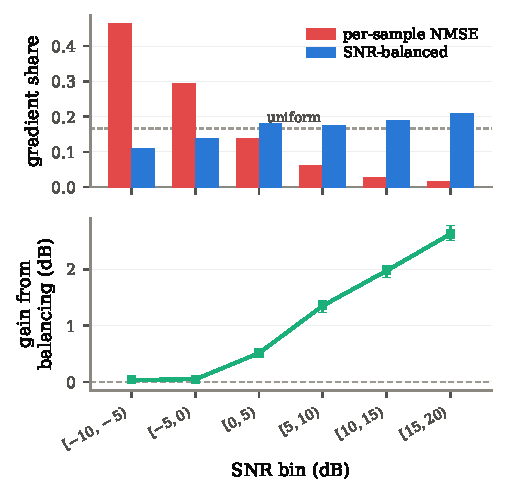
\includegraphics[width=\columnwidth]{fig/fig3_balanced_loss.pdf}
\caption{Cause and effect. Upper: per-bin gradient share under the per-sample
normalized loss and under SNR balancing. Lower: the resulting per-bin gain,
paired per-trial median with bootstrap $95\%$ CI.}
\label{fig:balanced}
\end{figure}

\subsection{Pilot efficiency is not pilot-count generalization}

A pilot-count curve for a trained estimator can mean two different things: one
model trained at some $P_0$ and evaluated at each $P$ (generalization), or a
model trained at each $P$ (efficiency). These are not close.
% src: reports/trackD_stage5_eval.json P14_P10
Trained at $P=10$, the estimator beats the $P=20$ model evaluated there by
$+2.231$~dB pooled, every bin's CI excluding zero. At $P=35$ the corresponding
margin is $+0.635$~dB, so the model generalizes upward in pilot count far
better than downward.

At $5$~dB the matched-trained estimator reaches
% src: reports/trackD_pilot_three_way.json
$-7.52$~dB at $P=10$, within $0.47$~dB of the genie-aided reference, while the
$P=20$ model evaluated there is $2.60$~dB short of it. The clearest single
indication that the curve is tied to its training condition is that the
$P=20$ model is \emph{worse} at $P=25$ ($-11.13$~dB) than at $P=20$
($-11.27$~dB): more measurements, worse estimate. Fig.~\ref{fig:pilots} shows
all three curves together.

This matters for how such curves are reported. The pilot sweep of
\cite{xiao2026} is specified only as ``evaluated at a fixed SNR of $5$~dB'';
the text does not state whether the networks were retrained per pilot count.
We report that as a fact about what the paper specifies, and as motivation for
stating the distinction explicitly --- not as a criticism of that work, whose
convention is the ordinary one and which our own earlier curves shared.

\begin{figure}[!t]
\centering
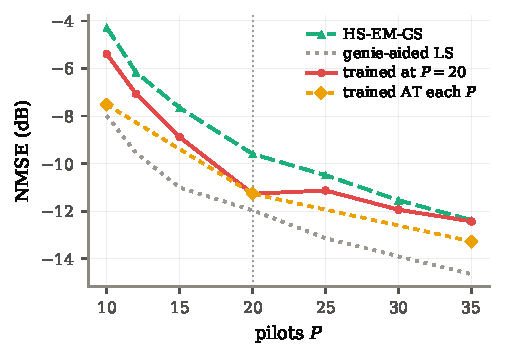
\includegraphics[width=\columnwidth]{fig/fig4_pilots_three_way.pdf}
\caption{Pilot efficiency against pilot-count generalization at $5$~dB, on
identical realizations. The dashed diamonds are separate networks trained at
each $P$; the solid curve is one network trained at $P=20$.}
\label{fig:pilots}
\end{figure}

\section{Conclusion}

Most of the apparent benefit of adding an explicit structural prior to an
unrolled channel estimator, in this setting, is an artifact of the training
convention rather than information supplied by the prior. Per-sample
normalized error over a mixed-SNR training set concentrates $89.7\%$ of the
gradient below $5$~dB and leaves the high-SNR regime underfitted; a prior that
helps there is credited with information it did not supply. Under a
matched-adequacy control the effect falls fifteenfold, from $+1.209$ to
$+0.078$~dB. Rebalancing the loss --- a change of a few lines, no
architectural addition --- recovers $+1.902$~dB at SNR~$\ge5$~dB at no
low-SNR cost, considerably more than the prior appeared to offer. We recommend
the control be run before a structural prior is credited, and note that it
cost us our own result first.

\textbf{Limitations.} All results are simulation only, with no measured
hardware and no recorded channel data. They cover the geometric ULA model of
\eqref{eq:fwd} at $N=32$, $K=3$, one data budget and the pilot counts tested;
the negative result about structural priors is scoped to those conditions and
is not a general claim. We establish no fundamental bound: the reference curve
used throughout is genie-aided, presumes phase no receiver observes, and is
passed by our own estimator at low SNR.

\bibliographystyle{IEEEtran}
\bibliography{refs}

\end{document}
